\documentclass[a4paper]{article}

\usepackage[english]{babel}
\usepackage[utf8]{inputenc}
\usepackage{amsmath}
\usepackage{graphicx}
\usepackage[linktocpage]{hyperref}
\usepackage[colorinlistoftodos]{todonotes}
%% \usepackage{here}
\usepackage{comment}
\usepackage[format=plain,labelfont=sc]{caption}
\usepackage{subfig}
\usepackage{array,multirow,makecell}
\usepackage{fancyhdr}
\usepackage{cite}
\usepackage{color,soulutf8}
\usepackage[nottoc,numbib]{tocbibind}

%% notes
%% commands
\newcommand{\mynotes}[1]{\textcolor{red}{#1}}
\newcommand{\addref}[1]{\todo[color=pink!40]{#1}}
\newcommand{\add}[1]{\todo[color=cyan!40]{#1}}
\newcommand{\remove}[1]{\todo[color=red!40]{#1}}
\newcommand{\rewrite}[1]{\todo[color=green!40]{#1}}
\newcommand{\hladdref}[2]{\hl{#1} \addref{#2}}
\newcommand{\hladd}[1]{\sethlcolor{cyan} \hl{#1} \add{#1}}
\newcommand{\hlremove}[1]{\sethlcolor{red} \hl{#1} \remove{#1}}
\newcommand{\hlrewrite}[2]{\sethlcolor{green} \hl{#1} \rewrite{#2}}
\newcommand{\hlcomment}[2]{\sethlcolor{orange} \hl{#1} \todo{#2}}
%%

\pagestyle{fancy}

\fancypagestyle{plain}{
\fancyhf{}
  \lfoot{
\includegraphics[width=0.2\textwidth]{Titre/insa-couleur.png}} 
  \cfoot{
\includegraphics[width=0.2\textwidth]{Titre/logo.jpg}}
  \rfoot{
\includegraphics[width=0.2\textwidth]{Titre/logo2.png}}
  \renewcommand{\headrulewidth}{0pt}
}

\newcommand{\HRule}{\rule{\linewidth}{0.5mm}}

\makeatletter
\newcommand*{\centerfloat}{%
  \parindent \z@
  \leftskip \z@ \@plus 1fil \@minus \textwidth
  \rightskip\leftskip
  \parfillskip \z@skip}
\makeatother

\title{Rapport de stage}

\begin{document}

\begin{titlepage}

\begin{center}

\thispagestyle{plain}

{ \Huge \textsc{Rapport de stage}\  \\[0.4cm] }
\HRule \\[0.4cm]
{ \Large Assemblage \textit{de novo} des génomes mitochondriaux et chloroplastiques de 10 accessions naturelles d'\textit{Arabidopsis thaliana}  \\[0.4cm] }
\HRule \\[0.4cm]

\vspace{1.5cm}

% Author and supervisor
\begin{minipage}{0.4\textwidth}
\begin{flushleft} \large
\emph{Auteur}\\
Myriam \textsc{Shafie}
\end{flushleft}
\end{minipage}
\begin{minipage}{0.4\textwidth}
\begin{flushright} \large
	\emph{Tuteur} \\
	\mynotes{il me semble que tu as 3 encadrants} \\
	Fabienne \textsc{Granier} \\
	\mynotes{Delphine Charif} \\
	\mynotes{Joseph Tran}
\end{flushright}
\end{minipage}

\vspace{2cm}

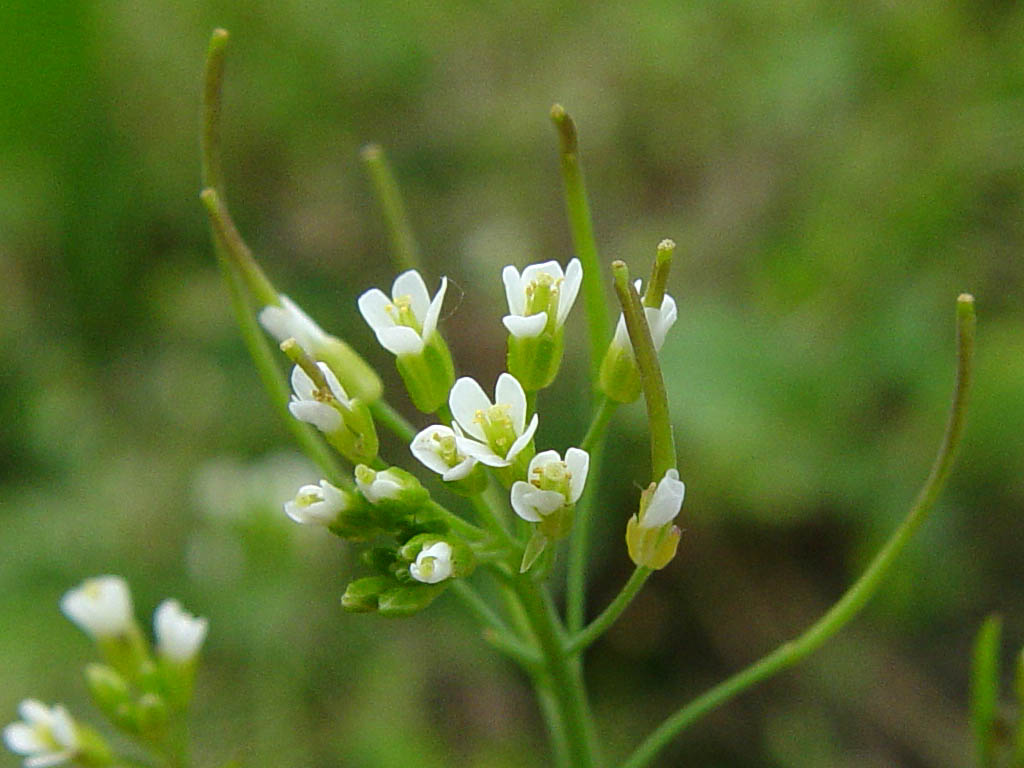
\includegraphics[scale=0.2]{Titre/a_thaliana.jpg}

\vspace{1cm}

Equipe Bioinformatique et Informatique \\[0.2cm]
Institut Jean-Pierre Bourgin \\[0.2cm]
INRA Centre de Versailles-Grignon


\end{center}

\end{titlepage}

\section*{Remerciements}

\newpage

\renewcommand{\contentsname}{Table des matières} 

\cleardoublepage
\pdfbookmark{\contentsname}{toc}
\tableofcontents

%% notes todolist
%% \todototoc 
\listoftodos
%%

\newpage

\section{Présentation de l'organisme d'accueil}

L'Institut Jean-Pierre Bourgin est une unité mixte de recherche INRA-AgroParisTech consacrée à l'étude de la biologie végétale. Il comporte environ 350 personnes, réparties en 25 équipes.

Les thématiques étudiées à l'IJPB sont très variées. Elles sont regroupés en 5 grands pôles : 
\begin{itemize}
\item Morphogenèse, Signalisation, Modélisation 
\item Dynamique et expression des génomes 
\item Adaptation des plantes à leur environnement 
\item Reproduction et Graines 
\item Paroi végétale, fonction et usage
\end{itemize}

J'ai réalisé mon stage au sein de l'équipe Bioinformatique et Informatique. 

%il manque des choses ici

\section{Introduction}

\subsection{Mise en situation biologique}

Les plantes vertes possèdent trois compartiments génétiques : le noyau, la mitochondrie (mt) et le chloroplaste (ct). La mitochondrie et le chloroplaste étaient à l'origine des bactéries endosymbiotes ; elles ont été intégrées à la cellule végétale lors de l'évolution et sont devenus des organites cellulaires. Au cours de cette intégration, une grande partie des génomes mt et ct a été transféré vers le noyau. 

Cependant, la mitochondrie et le chloroplaste conservent un petit nombre de gènes cruciaux à leur fonctionnement. Ces gènes ne se suffisent bien évidemment pas à eux-mêmes. Les produits codés par le noyau et par les organites doivent absolument interagir entre eux pour que la mitochondrie et le chloroplaste fonctionnement correctement. 

Ainsi, une co-évolution du génome nucléaire et cytoplasmique paraît obligatoire, car un changement dans l'un doit forcément être \hlrewrite{refléter}{reflété} par un changement dans l'autre afin de perpétuer leur interaction. Ce mécanisme fait que les génomes du noyau et des organites vont s'adapter à l'environnement de manière coopérative.

La figure \ref{coadaptation} illustre ce principe. Il présente trois étapes de l'histoire évolutive d'une plante. Initialement, la plante possède l'allèle \hlrewrite{ancestrale}{ancestral} N0 pour un gène du noyau et l'allèle \hlrewrite{ancestrale}{ancestral} C0 pour un gène d'un des organites. Les produits de ces deux gènes interagissent correctement au niveau physiologique. Cet interaction contribue à la fitness globale de la plante et à son phénotype.

Le gène cytoplasmique subit alors une mutation. La plante possède l'allèle \hlrewrite{dérivée}{dérivé} C1 pour le gène cytoplasmique mais toujours l'allèle \hlrewrite{ancestrale}{ancestral} N0 pour le gène nucléaire. L'interaction des produits des deux gènes est toujours possible mais elle est un peu moins efficace au niveau physiologique. Cependant, la fitness globale de la plante n'est pas diminuée, par exemple parce que la mutation C1 permet à la plante de s'adapter à un changement dans son environnement. \hlcomment{La mutation C1 va donc être fixée.}{Un peu trop déterministe} 

Enfin, une mutation N1 du gène nucléaire va être positivement sélectionnée. En effet, cette mutation permet de restaurer une interaction optimale entre les produits des gènes nucléaire et cytoplasmique au niveau physiologique. Les gènes nucléaire et cytoplasmique ont donc évolués \hlrewrite{main dans la main}{conjointement} pour assurer l'adaptation de la plante à son nouvel environnement. 

\begin{figure}[!ht]
\centering
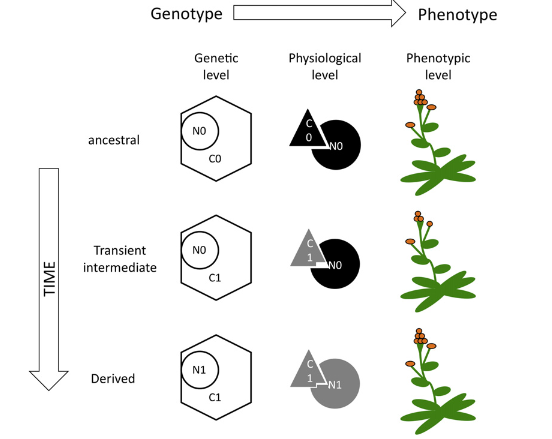
\includegraphics[scale=0.8]{Introduction/coadaptation.PNG}
\caption{La coadaptation nucléo-cytoplasmique \cite{marechal2012mitochondrial}}
\label{coadaptation}
\end{figure}

Le meilleur moyen de mettre en évidence expérimentalement la coadaptation nucléo-cytoplasmique est de la briser.

Considérons deux plantes d'une même espèce (donc interfertiles) mais appartenant à deux sous-espèces différentes ayant divergées depuis longtemps (par exemple, une plante poussant en France et une autre aux Etats-Unis). Le cytoplasme et le noyau de ces deux plantes ne sont pas compatibles. 

On peut obtenir par croisements une plante qui possède le génome nucléaire de l'une et le génome cytoplasmique de l'autre. On mesure ensuite les caractéristiques phénotypiques qui nous intéressent chez la plante et ses parents. On peut ainsi repérer et quantifier l'influence de la coadaptation nucléo-cytoplasmique sur ces traits. 

\subsection{Le projet CytoPhéno}

Le projet CytoPhéno (signifiant \textit{Co-adaptation nucléo-cytoplasmique et phénotypes adaptatifs des plantes}) a été mis en place en 2012. Il est piloté par Françoise Budar, directrice de l'équipe Organites et Reproduction de l'IJPB, mais il implique également de \hlrewrite{nombreuses}{nombreux} autres partenaires de l'INRA et du CNRS. 

Ce projet possède deux volets de recherche, bien évidemment liés : la co-adapatation nucléo-cytoplasmique et le rôle du cytoplasme dans l'adaptation de la plante à son environnement. 

La plante choisie pour l'étude de ces thèmes est \textit{Arabidopsis Thaliana}. En effet, outre tous les avantages qui font d'\textit{Arabidopsis} un organisme modèle (petit génome, cycle de vie rapide etc.), cette plante possède une forte diversité génétique et est présente naturellement dans un très grand nombre d'habitats naturels, ce qui en fait une référence pour les études portant sur l'adaptation. De plus, les chercheurs de l'IJBP ont mis en évidence en 2010 l'existence de la co-adaptation nucléo-cytoplasmique chez \textit{Arabidopsis Thaliana}.\cite{moison2010cytoplasmic}

Ils ont choisi de concentrer leur étude sur la plus petite core collection (n=8) disponible au \textit{Versailles Arabidopsis Stock Center}. Une core collection est un petit groupe d'accessions naturelles d'\textit{Arabidopsis Thaliana} qui capture au mieux la diversité génétique et morphologique de l'espèce.\cite{mckhann2004nested}

A partir de ces 8 accessions naturelles, les chercheurs ont crée 56 cytolignées, représentant toutes les combinaisons noyau/cytoplasme possibles. 

Le projet CytoPhéno comporte différentes étapes.

\begin{enumerate}
	\item l'étude des \hlrewrite{variantes}{variations} \hladd{génomiques et} génétiques mitochondrial et chloroplastique pour les 8 accessions naturelles
\item la production d'un grand nombre de graines pour les accessions naturelles et les cytolignées
\item l'identification des gènes nucléaires et cytoplasmiques impliqués dans la co-adaptation  
\item le phénotypage de la core collection et des cytolignées pour différents traits (germination, réponse à différents niveaux de nitrogène etc.)
\item l'analyse statistique des résultats afin d'évaluer l'effet sur le phénotype du noyau, du cytoplasme et de l'interaction nucléo-cytoplasmique
\end{enumerate}

Suite à ces tâches, nous pourrons répondre aux questions suivantes :  

Quels phénotypes sont impactés quand la co-adaptation nucléo-cytoplasmique est rompue ? Et quels gènes sont impliqués ?

Quels traits potentiellement adaptatifs sont modifiés par des variations du génome cytoplasmique ? A quel point ces traits sont également impactés par la co-adaptation nucléo-cytoplasmique ?  

\subsection{La tâche 1 : Analyse bioinformatique}

Lors de mon stage, j'ai travaillé sur la première tâche du projet CytoPhéno : l'analyse des génomes mitochondriaux et chloroplastique des 8 accessions naturelles.

Le but de \hlrewrite{cet}{cette} tâche est de trouver des polymorphismes non neutres entre les différentes accessions. En effet, les gènes présents dans des versions significativement différentes selon les accessions sont peut-être impliqués dans la rupture de la coadaptation nucléo-cytoplasmique. 

Pour trouver ces variants, il va falloir aligner ou assembler les génomes mitochondriaux et chloroplastiques des 8 accessions puis les annoter. 

Les mitochondries des plantes évoluent peu par mutations ponctuelles et beaucoup par réarrangements. Des pans entiers de génomes vont donc être réordonnées entre nos 8 accessions naturelles et la référence dont nous disposons (génome mitochondrial de l'accession C24). On privilégie donc l'assemblage \textit{de novo} par rapport à l'alignement pour la mitochondrie.

Le chloroplaste présente lui beaucoup de SNPs et peu de réarrangements. On pourrait donc l'aligner à une référence. Cependant, les données dont nous disposons contiennent à la fois les génomes mt et ct. Séparer les deux génomes est difficile car il y a des insertions du génome chloroplastique dans la mitochondrie et vice-versa. Les bioinformaticiens de l'IJPB ont donc \hlrewrite{optés}{opté} pour un assemblage \textit{de novo} simultané des génomes mt et ct.


\section{Matériels et méthodes}

\subsection{Les données brutes}

Nous disposons de 10 librairies de reads correspondant chacune à une accession. 

\begin{table}[!ht]
\centering
\begin{tabular}{|l|l|}
\hline
   Nom & Habitat \\
   \hline
   Jea & St-Jean Cap Ferrat [France] \\
   Ita-0 & Ibel Tazekka (Jebel Tazekka) [Maroc] \\
   Cvi-0 & Cap-Vert [Cap-Vert] \\
   Bur-0 & Burren [Irlande] \\
   Blh-1 & Bulhary [République Tchèque] \\
   Oy-0 & Oystese [Norvège] \\
   Sha(hdara) & Shakdara River (Pamir) [Tadjikistan] \\
   Ct-1 & Catane [Italie] \\
   Mr-0* & Monterosso [Italie] \\
   Kz-9* & Atasu [Kazakhstan] \\
   \hline
\end{tabular}
\label{donnees}
\caption{Présentation des 10 accessions étudiées (* : ne fait pas partie de la core collection)}
\end{table}

Outre les 8 membres de la core-collection, nous avons également étudié les génomes des accessions Mr-0 et Kz-9 d'\textit{Arabidopsis Thaliana}. Ces deux accessions ont été ajoutées par Françoise Budar, la coordinatrice du projet, car elle présente un intérêt particulier pour son étude de la stérilité mâle cytoplasmique (recherche des gènes cytoplasmiques qui induisent la stérilité mâle chez certaines accessions d'\textit{Arabidopsis Thaliana}). 

Les génomes mitochondriaux et chloroplastiques des 10 accessions ont été séquencés en paired-end, Sha et Kz-9 par la technologie Illumina HiSeq 2000 (2X100 bases) et toutes les autres accessions par la technologie Illumina MiSeq 2000 (2X150 bases). Nous avons donc, pour chaque accession, deux fichiers fastq contenant les reads pairés. 

\subsection{Préparation des séquences}

Avant d'aligner ou d'assembler ces reads, il est nécessaire d'effectuer une analyse de qualité. Elle nous permettra de détecter d'éventuelles contaminations de la librairie ou des problèmes de séquençage (par exemple, une mauvaise qualité d'imagerie sur une flowcell va donner un sous-ensemble de reads de mauvaise qualité).

On effectue l'analyse de qualité avec fastqc. Cet outil possède plusieurs modules qui vont chacune évaluer un indicateur : la qualité des bases (selon leur position sur le read), la longueur des reads etc. Chacune des ces mesures est comparée à ce qui est attendu pour une librairie aléatoire. Si l'observé et \hlrewrite{le prédit}{l'attendu} sont proches, le module est validé.

Si le module est rejeté, cela signifie que la librairie étudiée diffère sur ce point d'une librairie aléatoire. Cette différence peut provenir d'une contamination ou d'un biais de séquençage mais elle peut également résulter de la réalité biologique de nos données (qui ne sont, bien évidemment, pas aléatoires).

Il est donc nécessaire de regarder non seulement le résultats des tests (module validé, non validé ou à la limite de validation) mais aussi la sortie graphique de chaque module. fastqc fournit une représentation graphique de chaque indicateur testé : boxplot des qualités de chaque base selon leur position dans le read, abondance des reads en fonction de leur longueur etc. 

\hlcomment{Si les indicateurs sont normaux pour notre librairie, on peut procéder au nettoyage des reads. Pour cela, on utilise l'outil Trimmomatic.}{C'est à nuancer, le fait que des indicateurs soient au rouge, cela peut ou non poser problème mais certains peuvent être ignorés sans que cela impacte le reste de l'analyse}

Trimmomatic va supprimer aux extrémités 3' et 5' les bases dont la qualité est inférieure à 20 (ce qui signifie que la base a une chance sur cent d'avoir été mal identifiée). Puis, il fait glisser une fenêtre de 4 nucléotides sur la séquence : si la qualité moyenne de la fenêtre est inférieure à 15, elle est supprimée. Les reads devenus trop courts (moins de 50 bases) sont ensuite jetés.

Après trimming, on refait une analyse de qualité sur les reads \hlrewrite{retenus}{retenues} pour vérifier que le nettoyage a bien amélioré la qualité de la librairie.

\subsection{Alignement}

Avant d'effectuer l'assemblage \textit{de novo} de nos libraries nettoyées, on va d'abord les aligner à une référence : génome nucléaire et chloroplastique de l'accession Col-0 et génome mitochondrial de C24. 

Pourquoi cet alignement ? 

Il nous permettra : 
\begin{itemize}
\item de quantifier le degré de contamination nucléaire de notre librairie

\item d'évaluer la couverture pour chaque génome et chaque accession, ce qui est essentiel pour l'assemblage

\end{itemize}

Pour l'alignement, on utilise l'outil bwa. On autorise 2 événements indépendants seulement (par exemple, un mismatch plus un micro-indel). Ce critère stringent est adapté au génome mitochondrial, où il y a très peu de mutations ponctuelles.

Les alignements obtenus sont au format SAM, où \hlrewrite{chaque read correspond à une ligne.}{à chaque ligne correspond une read.} Si \hlrewrite{un}{une} read s'aligne à plusieurs endroits du génome, un seul alignement est choisi au hasard. Cela nous contraint à masquer le chromosome 2 de la référence. En effet,  la quasi-totalité de la mitochondrie est insérée à l'intérieur de ce chromosome.\cite{chr2} Donc, si nous ne le masquions pas, les reads mitochondriaux auraient un best hit sur la mitochondrie et un best hit sur le chromosome 2 et la moitié d'entre \hlrewrite{eux}{elles} environ seraient assigné au noyau. L'estimation de la couverture mitochondriale serait alors complètement faussée. 

\subsection{Réduction des jeux de données}

En une fois, on ne séquence par shotgun qu'une fraction aléatoire du génome. Pour être sur que nos reads couvrent 90\% et plus du génome, il est nécessaire d'échantilloner le génome un très grand nombre de fois. Certaines régions se retrouveront dans de nombreux échantillons et auront donc une forte couverture. D'autres se retrouveront dans peu d'échantillons et seront peu couvertes. Une minorité de reads seront donc cruciaux et une majorité de reads complètement redondants. 

Cette grande quantité de reads inutiles va poser des problèmes à l'assemblage. Le temps et la mémoire nécessaire pour les traiter sont non négligeables. De plus, ces reads contiennent des erreurs de séquençage. Si on les éliminait, la qualité de l'assemblage serait améliorée, particulièrement pour les assembleurs utilisant des graphes de \hlrewrite{Bruijn}{De Bruijn}, que les noeuds et les arrêtes erronés peuvent rapidement envahir quand les jeux de données sont trop gros.

On va tester deux approches pour réduire le jeu de données. \\

Premièrement, le ré-échantillonage. Il consiste simplement à tirer aléatoirement un échantillon dans la librairie. On choisit la taille de l'échantillon en fonction des couvertures mitochondrial et chloroplastique qu'on souhaite obtenir.

Par exemple, pour Cvi-0, les couvertures des génomes mitochondrial et chloroplastique ont été estimées par alignement à 60X et 560X pour le jeu de donnée brut. En ne conservant en moyenne qu'\hlrewrite{un}{une} read sur trois, nous devrions obtenir une couverture de 20X sur la mitochondrie et de 190X sur le chloroplaste. 

Nous ne connaissons pas \textit{à priori} quelles couvertures des génomes mt et ct \hlrewrite{vous}{vont} nous donner les meilleurs résultats. Nous sommes donc obligés de tester plusieurs valeurs, en gardant toutefois en tête que des couvertures très élevées (supérieures à 1000X) ont peu de chances de founir de bons assemblages.\\

Deuxièmement, la normalisation digitale. Cette procédure utilise la distribution de l'abondance des k-mers pour estimer la couverture par read et éliminer les reads dont la couverture dépasse la limite imposée.\cite{brown2012reference} Elle présente l'avantage, outre de réduire la taille du jeu de données, d'homogéiniser les couvertures des deux génomes.

On va normaliser les données avec khmer. Ce programme propose également un outil de filtration des données. Il permet de supprimer les reads contenant des k-mers d'abondance inférieure à la limite choisie. Ces k-mers de faible abondance correspondent à des erreurs de séquençage et, dans notre cas, à de la contamination nucléaire. On va donc appliquer une filtration après normalisation pour essayer de supprimer tous les reads correspondant au noyau. 

Les seuils de normalisation et de filtration ne sont pas connus au préalable. On est obligé de procéder par tâtonnements en testant plusieurs valeurs des paramètres. On vérifie que les jeux de données obtenus sont valides, c'est-à-dire que la couverture a bien été réduite et homogénéisée et que les données supprimées étaient bien redondantes.\\ 

Nous avons pour chaque accession plusieurs jeux de donnée réduits selon  différentes méthodes et différents paramètres. Nous devons les assembler afin de comparer la qualité des résultats obtenus pour chaque jeu de donnée. 

\subsection{Assemblage}

\subsubsection{Choix d'une stratégie d'assemblage}

Le premier problème auquel nous allons être confrontés est que nous n'assemblons pas un seul génome mais deux simultanément. Deux solutions s'offrent à nous : 
\begin{itemize}
\item utiliser un assembleur classique.

	Cette option n'est valable que \hladd{si} les jeux de données pour lesquels les couvertures des génomes mitochondrial et chloroplastique sont les mêmes (jeux de données normalisés). 

\item utiliser un assembleur de métagénome.

L'assembleur métagénomique va utiliser les différences de couverture pour distinguer 1) la mitochondrie du chloroplaste 2) les régions répétées des régions non répétées. On ne peut donc pas utiliser de jeux de données normalisé, pour lesquels la couverture a été rabotée en dessous d'une certaine limite. Pour cette approche, on ne se servira que de jeu de donnée ré-échantillonné, où les différentes couvertures ont été réduites tout en maintenant leur stoechiométrie.  

\end{itemize}

Pour l'assemblage classique, nous avons utilisé Velvet et SGA. En effet, ces deux assembleurs sont basés sur des principes différents : les graphes de \hlrewrite{Bruijn}{De Bruijn} pour Velvet et l'Overlap \hlrewrite{Consensus Layout}{Layout Consensus} pour SGA. SGA identifie toutes les paires de reads qui se recouvrent et construit un graphe avec un noeud pour chaque read et une arrête pour chaque paire de reads qui se recouvre. Le graphe est ensuite simplifiée (on retire les arrêtes redondantes) et stocké efficacement grâce à la transformée de Burrows-Wheeler. \cite{simpson2012efficient}

Notre assembleur de métagénome sera MetaVelvet. 

\hlcomment{A noter que Velvet et MetaVelvet n'ont assuré que la partie contiguage de l'assemblage}{À nuancer au vu de tes récents tests qui semble indiquer que pebble intervient dans le scaffolding meme quand il est explicitement non dema,dé à Velvet\dots}. La partie scaffolding a été effectuée par Bambus2. Pour SGA, nous avons utilisé son scaffolder intégré (sga scaffold). 

\subsubsection{Choix des paramètres pour Velvet et MetaVelvet}

L'un des paramètres les plus importants pour un assemblage par graphe de \hlrewrite{Bruijn}{De Bruijn} est la taille de k-mer utilisé pour construire le graphe. 

Nous avons \hlrewrite{construit}{implémenté} notre propre script pour lancer Velvet avec de multiples valeurs de k. Les deux options les plus importantes, outre la taille du k-mer, sont  \textit{exp\_cov} et \textit{cov\_cutoff}. 

\textit{exp\_cov} permet d'indiquer à Velvet la couverture attendue pour une région unique du génome. On aligne le jeu de données normalisé à la référence et on estime à nouveau les couvertures du chloroplaste et de la mitochondrie. On doit obtenir une valeur unique qu'on fournit à \textit{exp\_cov}. 

Les noeuds dont la couverture sont inférieure à \textit{cov\_cutoff} sont retirés du graphe de \hlrewrite{Bruijn}{De Bruijn} après sa construction. \todo{Je nuancerais l'efficacité du filtre\dots}\hlrewrite{Cette option permet donc d'éliminer toute trace de contamination nucléaire qui aurait échappé au filtrage.}{Cette option permet de réduire fortement la contamination nucléaire ou les erreurs qui auraient échappé à la normalisation.}  

Pour MetaVelvet, nous avons procédé exactement de la même façon. La seule différence est que l'option \textit{exp\_cov} est remplacée par \textit{exp\_covs}. On fournit à MetaVelvet les deux pics de couvertures qui correspondent à la mitochondrie et au chloroplaste.

La qualité des assemblages réalisés avec différents k est ensuite comparée à l'aide de Quast. Quast est un script Python qui va calculer les statistiques de chaque assemblage (N50, taille du plus grand contig etc.) et les présenter sous forme d'un rapport HTML pour une comparaison facile. On peut donc rapidement repérer la taille de k-mer qui semble produire le meilleur assemblage.

\subsubsection{Choix des paramètres pour SGA}

SGA propose un ensemble de programmes qui filtrent et trimment les reads, trouvent les recouvrements entre les reads, construisent le String Graph et créent les contigs. Pour effectuer ces étapes, on s'est fortement inspiré d'un des scripts bash proposés par les auteurs de SGA pour assembler le génome de \textit{C. Elegans}. %Le seul paramètre qu'on a changé est la longueur minimale de recouvrement entre deux reads, qu'on fixe à 2/3 de la longueur des reads (ie 100 pour des reads de 150 bases).

Pour le scaffolding, on réaligne le jeu de données sur les contigs avec \textit{sga align} et on utilise le fichier BAM obtenu 1)
pour avoir une liste des liens entre les contigs à l'aide du script Perl \textit{sga-bam2de} 2) pour calculer pour chaque contig la statistique de Myers avec le script Python \textit{sga-astat}. 

Cette statistique sera utilisé par \textit{sga scaffold} pour déterminer quels contigs correspondent à des répétitions : tous les contigs qui ont une statistique de Myers inférieure à un certain seuil sont considérés comme étant répétés. Pour déterminer le bon seuil, on compare les valeurs de la statistique de Myers pour les contigs chloroplastiques uniques et répétées (voir la structure du chloroplaste figure \ref{schemachloro}). On passe également à \textit{sga scaffold} les options \textit{--strict --remove-conflicting} pour avoir les scaffolds les plus conservatifs possibles. 

\textit{sga scaffold} donne pour chaque scaffold, la liste des contigs qui le constituent et comment ils sont placés les uns par rapport aux autres. \textit{sga scaffold2fasta} utilise ce fichier pour écrire la séquence des scaffolds au format fasta. On se place dans le mode résolution par graphe ; avec l'option \textit{-g best-any}, on tente de résoudre les gaps entre les contigs en parcourant le graphe et en trouvant le chemin qui correspond le mieux aux distances estimées entre les contigs. 

\subsubsection{Choix des paramètres pour Bambus2}

Bambus2 est une suite de scripts qui effectuent les différentes étapes du scaffolding. 

On commence par créer des liens entre les contigs (clk) puis on rassemble ces liens entre une collection de bord possibles pour les contigs (Bundler). Bambus2 nous permet également de repérer les régions répétées du génome (MarkRepeats). On  utilise ces informations pour placer les contigs les uns par rapport aux autres et les orienter (OrientContigs). Les scaffolds obtenus sous forme de graphe sont ensuite linéarisés et enregistrés au format fasta.  

Les deux étapes qui proposent des options intéressantes sont MarkRepeats et OrientContigs. 

%il manque des choses ici

\subsubsection{Choix des paramètres pour SGA}

On a fixé la longueur maximale d'une répétition à 20 000 bases. Pour choisir le seuil de la statistique de Myers, on procède comme expliqué précédemment pour SGA : on calcule la statistique de Myers pour chaque contig avec \textit{sga-astats}. On sait quels contigs chloroplastiques sont uniques et lesquels sont répétés (voir section suivante). On prend un seuil qui va permettre à Bambus2 de les ranger dans la bonne catégorie. 

\subsubsection{Evaluation de la qualité des assemblages obtenus}

\vspace{0.2cm}

Comment savoir si nos assemblages sont bons ou pas ? \\

\textbf{Pour le chloroplaste, on sait exactement ce que l'on doit obtenir}. Le chloroplaste évolue non par réarrangements mais par mutations ponctuelles. Les chloroplastes des 10 accessions naturelles vont donc être très proches du chloroplaste de référence. \\

Nous avons donc commencé par étudier la structure du chloroplaste de référence. 

On aligne le chloroplaste de référence contre lui-même à l'aide de Nucmer. Nucmer est \hlrewrite{une}{un} pipeline de la suite MUMmer qui permet d'aligner extrêmement rapidement des génomes entiers contre une référence et de représenter ces alignements sous forme de graphe de ressemblance (dotplots).  

\begin{figure}[!ht]
\centering
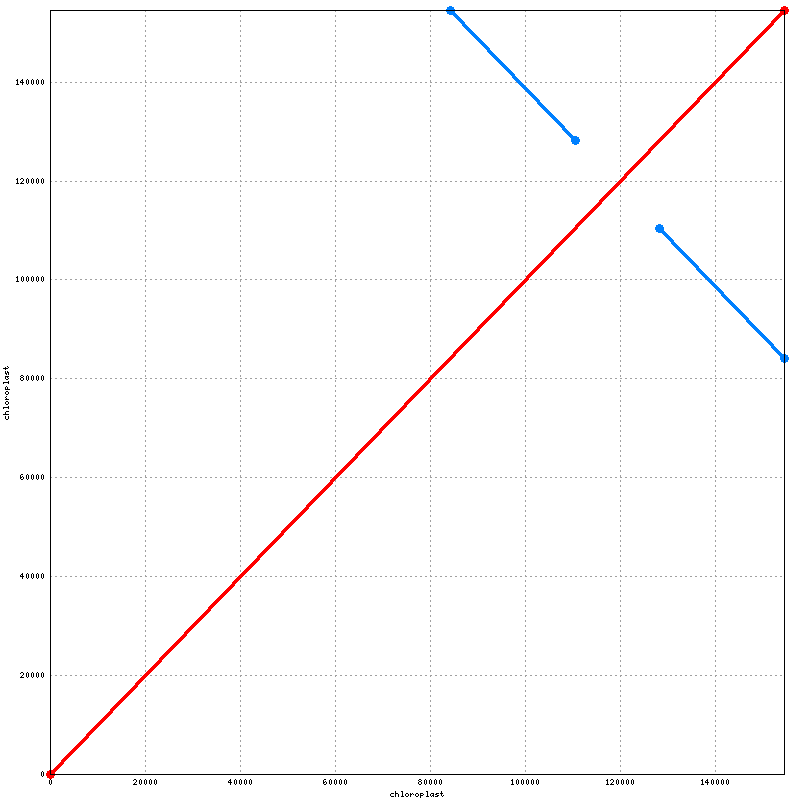
\includegraphics[scale=0.3] {Assemblage/chloroVSchloro.png}
\caption{Dotplot du chloroplaste de référence aligné contre lui-même}
\label{temoinchloro}
\end{figure}

La figure \ref{temoinchloro} met en évidence qu'une portion du chloroplaste de référence comprise entre 85 et 110kb est répétée et inversée entre 128 et 154kb. On devrait retrouver la même inversion-répétition chez les chloroplastes des dix accessions naturelles. 

\begin{figure}[!ht]
\centering
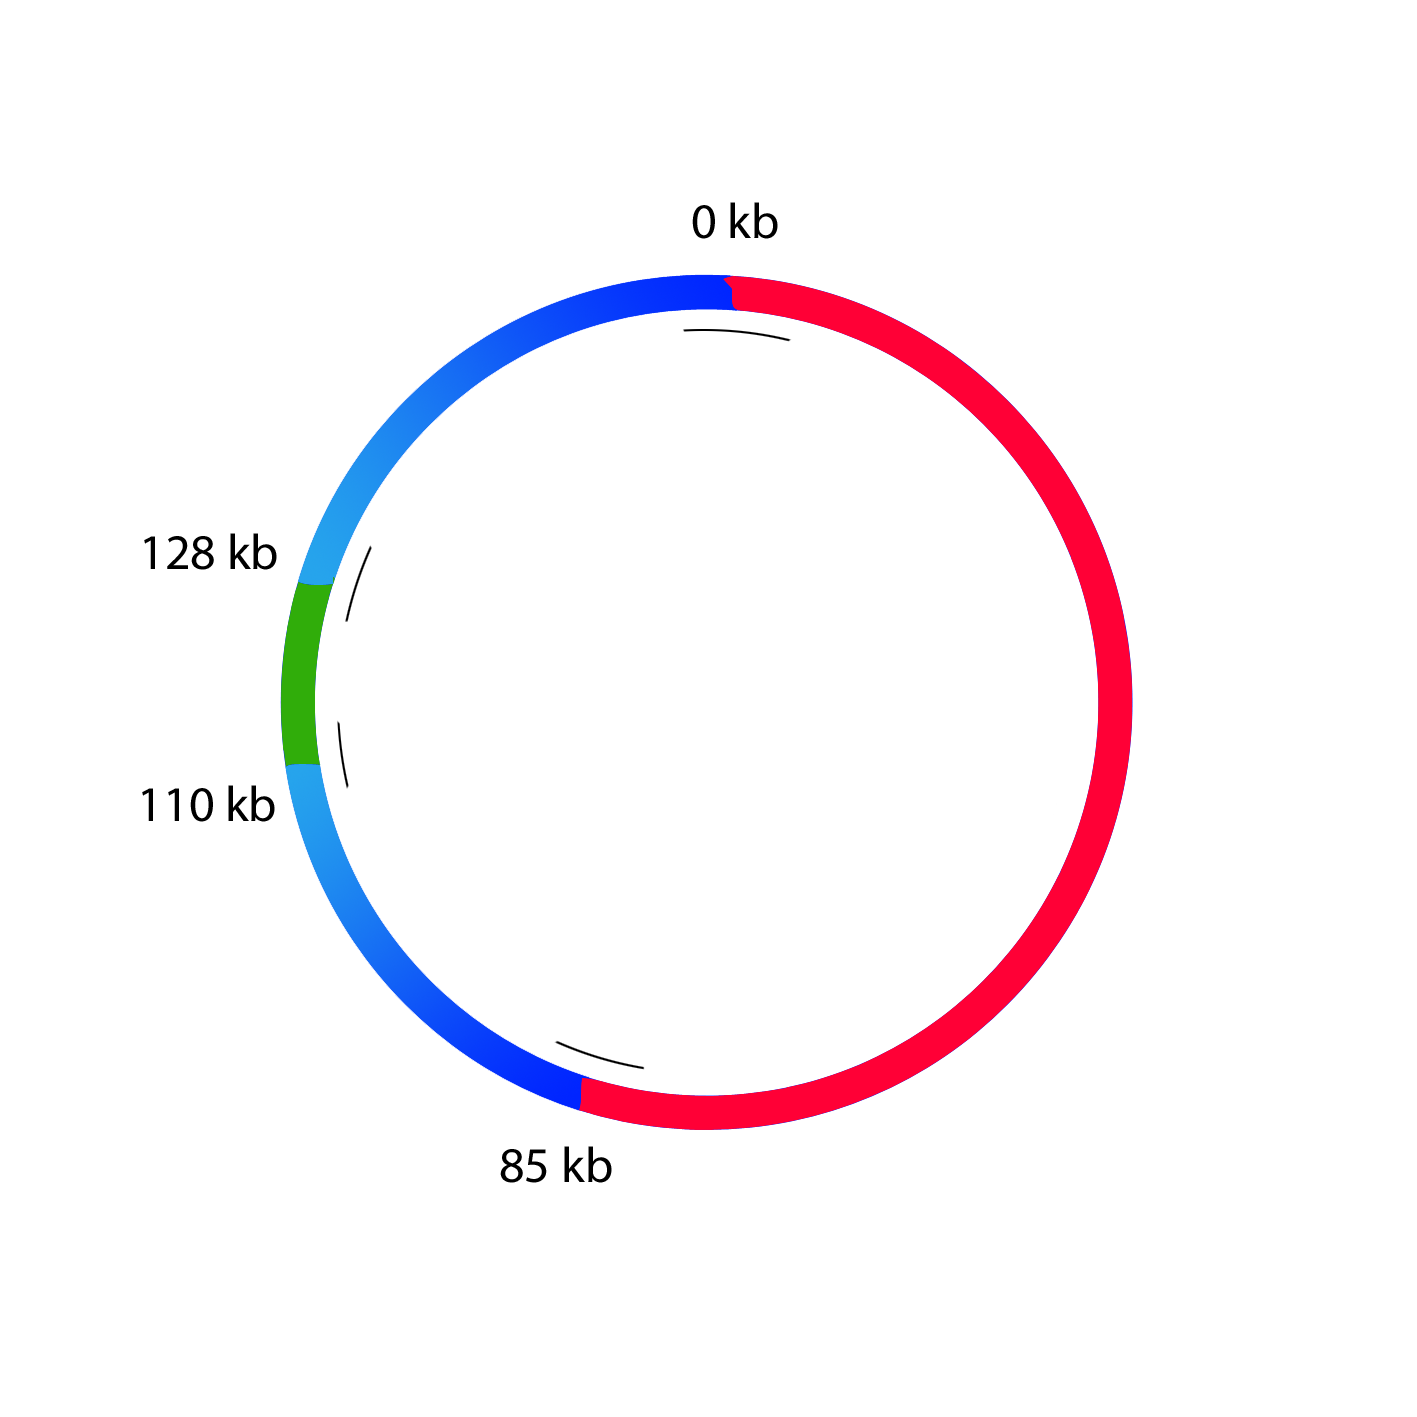
\includegraphics[scale=0.8] {Assemblage/schemachloro.png}
\caption{Structure du génome chloroplastique chez \textit{Arabidopsis Thaliana}, toutes accessions confondues}
\label{schemachloro}
\end{figure}

\textbf{Après contigage}, on aligne nos contigs contre le chloroplaste de référence à l'aide de Nucmer.  On doit obtenir :
\begin{itemize}
\item un contig non chimérique qui mappe sur le chloroplaste de référence entre 0 et 85kb dans le sens direct (en rouge sur la figure \ref{schemachloro})
\item un contig non chimérique  qui mappe sur le chloroplaste de référence entre 85 et 110kb dans le sens direct et entre 128 et 154kb dans le sens inverse (en bleu sur la figure \ref{schemachloro})
\item un contig non chimérique  qui mappe sur le chloroplaste de référence entre 110 et 128kb dans le sens direct (en vert sur la figure \ref{schemachloro})
\end{itemize}

Le contiguer ne sait pas que la région représentée en bleue est une région répétée. Il voit seulement qu'à ses extrémités existe plusieurs possibilités. Par exemple, l'extrémité bleu foncé de la région répétée est reliée aux deux extremités de la région unique rouge. Le contiguer ne doit pas faire un choix et fusionner les contigs bleu et rouge dans un sens ou dans l'autre. Il doit les garder séparés. 

Le scaffolder, en revanche, détecte les régions répétées et est censé les résoudre en théorie. En pratique, il est très difficile de résoudre de grandes inversions-répétitions comme celle qui se trouve sur le chloroplaste sans plusieurs librairies possédant des tailles d'inserts différentes. On s'estimera donc satisfait si les parties uniques du chloroplaste ont été correctement assemblées.

\textbf{Après scaffolding}, on doit donc avoir deux scaffolds non chimériques correspondant à la grande et la petite région unique du chloroplaste. \\

\textbf{Pour la mitochondrie, on ne sait pas précisément ce qu'on doit obtenir.} \hl{En raison des nombreux réarrangements qu'elles ont subis, les mitochondries des 10 accessions naturelles vont être très différentes}\todo[inline]{Je nuancerais vu que tu viens d'écrire que tu ne savais pas forcément ce qu'on allait obtenir puis de manière affirmative tu dis que ce sera très différent: je dirais qu'il est possible que les génomes mito soient différents vu qu'on étudie la core 8 qui est censé couvrir la variabilité naturelle la plus large}. \cite{arrieta2009diversity} Si on retrouve le même contig mitochondrial chez 9 accessions sur 10, cela ne signifie pas que l'assemblage de la dixième accession est mauvais. On peut néanmoins effectuer plusieurs tests afin de savoir si notre assemblage mitochondrial est plausible ou pas. 

\begin{enumerate}
	\item Avec Nucmer, on aligne les contigs ou les scaffolds contre la mitochondrie de référence afin de savoir si notre assemblage couvre la totalité \hlrewrite{de la mitochondrie}{du génome}. 

	\item On aligne les données brutes sur les contigs ou les scaffolds et on regarde si les contigs mitochondriaux et chloroplastique ont la couverture attendue (\hlrewrite{consistence}{consistance} interne).

\item On regarde si des paires s'alignent sur le même contig avec des tailles d'insert incohérentes. S'il y en a beaucoup, cela signifie que la structure interne du contig est mauvaise. On peut ainsi repérer et quantifier les mauvais contigs.

Pour compter le nombre de "mauvaises" paires dans chaque contig, on utilise la librairie R ContigLink. 

\end{enumerate}

ContigLink prend en entrée l'alignement au format bam des données brutes sur les contigs. Il sépare les \hlrewrite{pairs}{paires} qui s'alignent sur un seul et même contig et les \hlrewrite{pairs}{paires} \hlrewrite{qui s'alignent}{dont la read et la mate s'alignent} sur deux contigs différents. \hlrewrite{Ces deux types de}{Pour chacune de ces 2 catégories de} \hlrewrite{pairs}{paires} \hlremove{vont être utilisés pour calculer deux estimations de} la taille d'insert et \hlremove{de} son écart-type \hladd{sont estimés}. ContigLink donne ensuite une estimation de la qualité de l'assemblage. Cette estimation contient : 
\begin{itemize}
\item pour chaque contig, le nombre de \hlrewrite{pairs}{paires} s'alignant sur ce contig avec une bonne taille d'insert et une mauvaise taille d'insert (éloignée de son estimation par plus de deux écarts-type)
\item pour chaque \hlrewrite{pairs}{paires} de contigs, le nombre de "bonnes" et mauvaises" paires supportant un lien entre ces contigs.
\end{itemize}

Cette dernière information est très utile pour comprendre comment Bambus2 et sga scaffold vont relier les contigs entre eux pour former des scaffolds. 

\section{Résultats}

\subsection{Préparation des séquences}


\begin{figure}[!ht]
\centering

\subfloat[Avant trimming]{
   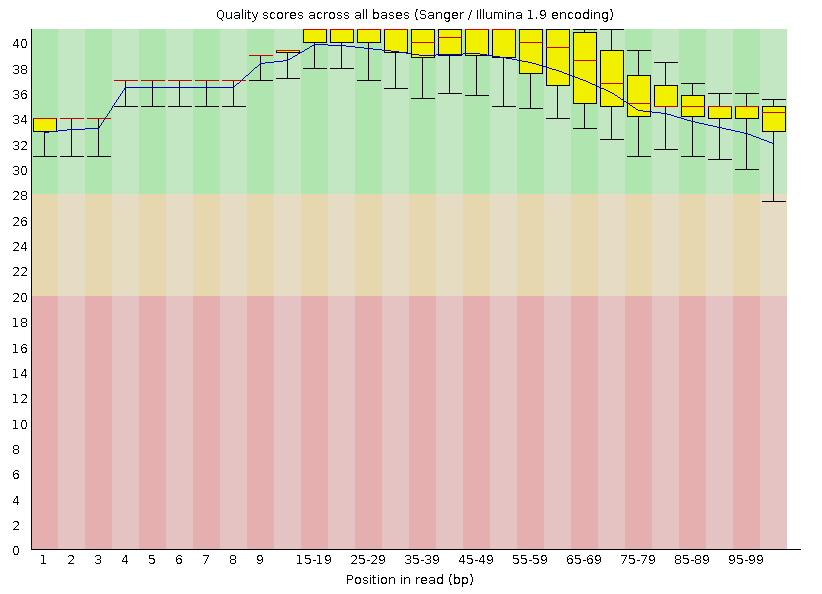
\includegraphics[scale=0.4] {Prep/QualitySha/avant1.png}
   \label{quality:1}
 }
 
\subfloat[Après trimming]{
   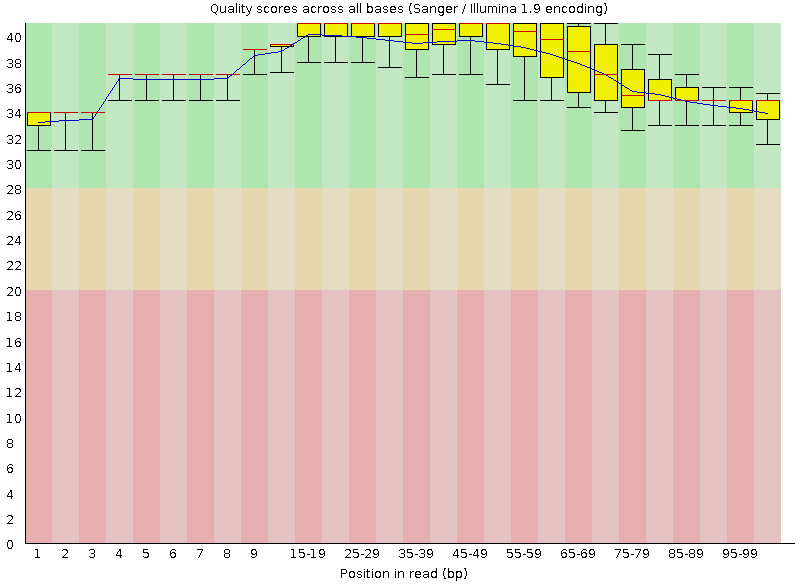
\includegraphics[scale=0.4] {Prep/QualitySha/apres1.png}
   \label{quality:2}
 }

\label{quality}
\caption{Qualité des bases en fonction de leur position sur les reads : exemple de Shahdara}
\end{figure}

La qualité de nos reads était excellente à la base : elle n'est donc que légèrement améliorée par le trimming. 

La quasi-totalité des séquences ont \hladd{été} conservé après trimming une taille proche de leur taille initiale  (autour de 100 bases pour Shahdara et Kz-9 et de 150 bases pour les autres accessions). 

Le taux de duplication de nos libraries est considéré comme trop élevé par fastqc. Cependant, comme notre librarie contient contient des données mitochondriales, où les séquences répétées sont fréquentes, nous n'avons pas à nous alarmer de ce résultat. 

\subsection{Alignement}

\begin{table}[!ht]
\centering
\begin{tabular}{|l|cccc|}
  \hline
 & Chloroplaste & Mitochondrie & Noyau & Non aligné \\ 
 \hline
Blh-1 & 8.08 & 64.26 & 15.26 & 12.40 \\ 
  Bur-0 & 16.16 & 9.78 & 42.79 & 31.26  \\ 
  Ct-1 & 16.09 & 6.32 & 45.20 & 32.39  \\ 
  Cvi-0 & 22.86 & 5.73 & 40.02 & 31.39  \\ 
  Ita-0 & 14.70 & 43.72 & 21.48 & 20.09  \\ 
  Jea & 12.83 & 21.90 & 38.84 & 26.43  \\ 
  Kz-9 & 15.86 & 21.02 & 44.15 & 18.98  \\ 
  Mr-0 & 8.04 & 66.05 & 13.07 & 12.84  \\ 
  Oy-0 & 15.86 & 11.04 & 42.97 & 30.12 \\ 
  Sha & 19.35 & 33.42 & 32.85 & 14.37 \\ 
  \hline
\end{tabular}
\caption{Pourçentage de reads mappées et non mappées pour les 10 accessions (référence sans chromosome 2)}
\end{table}
\todo{corrigé mappés par mappées}

Nous observons d'abord un pourcentage non négligeable de reads non \hlrewrite{mappés}{mappées} - jusqu'à 32\% pour l'accession Ct-1. 

\hlrewrite{Certains}{Certaines} reads non \hlrewrite{mappés}{mappées} appartiennent au chromosome 2 hors insertions mitochondriales. Comme le chromosome 2 est entièrement masqué, \hlrewrite{ils}{elles} ne peuvent s'aligner nulle part. 

D'autres correspondent à des régions où la variabilité entre l'accession étudiée et la référence dépasse le seuil fixé. On rappelle qu'avec les paramètres qu'on a fixé, pour qu'une read s'aligne à la référence, \hlrewrite{ils}{elles} doivent être \hlrewrite{séparés}{séparées} par moins de deux événements indépendants. Or, on a trouvé dans \hlrewrite{certains}{certaines} reads non \hlrewrite{mappés}{mappées} jusqu'à 7 SNPs de différence par rapport à la référence.\todo[inline]{En fait il faut regarder la paire, bwa peut sauver la mate avec un nombre d'événements indépendants supérieurs à la limite qu'on autorise si la read mappe en respectant les contraintes} 

Enfin, les autres reads non \hlrewrite{mappés}{mappées} ont une faible complexité et correspondent probablement à des régions répétées. \\

A partir du nombre de reads \hlrewrite{mappés}{mappées} sur chaque génome, on peut avoir une estimation de la couverture par une formule très simple : 

couverture $\approx$ nombre de reads \hlrewrite{mappés}{mappées} X taille des reads / taille du génome

\begin{table}[!ht]
\centering
\begin{tabular}{|l|ccc|}
  \hline
 & Chloroplaste & Mitochondrie & Noyau \\ 
  \hline
Kz-9 & 2845.83 & 1587.55 & 10.60 \\ 
  Sha & 2764.37 & 2010.17 & 6.28 \\ 
  Blh-1 & 218.26 & 730.76 & 0.55 \\ 
  Bur-0 & 466.26 & 118.79 & 1.65 \\ 
  Ct-1 & 348.44 & 57.65 & 1.31 \\ 
  Cvi-0 & 558.13 & 58.94 & 1.31 \\ 
  Ita-0 & 396.71 & 496.72 & 0.78 \\ 
  Jea & 326.96 & 235.05 & 1.33 \\ 
  Mr-0 & 237.68 & 822.04 & 0.52 \\ 
  Oy-0 & 458.24 & 134.26 & 1.66 \\ 
   \hline
\end{tabular}
\caption{Les couvertures par accessions (référence sans chromosome 2)}
\end{table}

Pour toutes les accessions, la couverture du noyau est faible devant celles de la mitochondrie et du chloroplaste. Cependant, le génome nucléaire d'\textit{Arabidopsis Thaliana} est 300 fois plus grand que le génome mitochondrial et 1000 fois plus grand que le génome chloroplastique. En nombre de bases, la contamination nucléaire est donc non négligeable et nous devrons nous efforcer de l'éliminer du jeu de données avant l'assemblage. 

Les couvertures mitochondriale et chloroplastique ne sont pas homogènes pour une même accession. Cela va nous poser problème car la taille de k-mer optimale pour l'assemblage par graphe de \hlrewrite{Bruijn}{De Bruijn} dépend de la couverture. On n'aura donc pas le même k-mer optimal pour les génomes mitochondrial et chloroplastique. Nous prendrons en compte cette disparité de couverture pour notre stratégie d'assemblage.

\begin{comment}
On visualise les alignements à l'aide du logiciel IGV. Sur la mitochondrie, on peut repérer visuellement de grands réarrangements.

\begin{figure}[!ht]
\centering
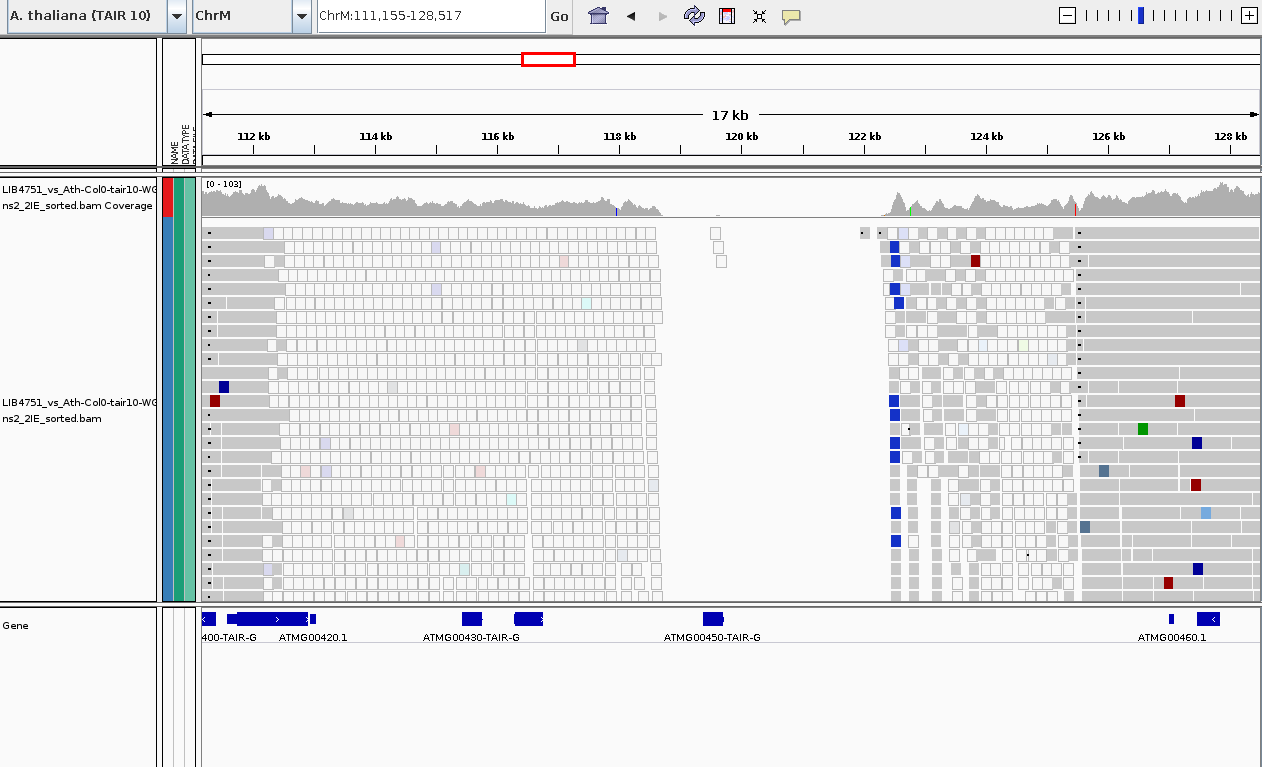
\includegraphics[scale=0.25]{Alignement/rearrangement-cvi0.png}
\label{rearrangement}
\caption{Un possible réarrangement sur le génome mitochondrial de Cvi-0 : on repère une zone où aucun read n'a mappé entourée de zones avec des reads de mauvaise qualité (en blanc) et des reads qui ont une mauvaise taille d'insert (en bleu et en rouge)}
\end{figure}

Nous avons comptabilisé ces réarrangements et noté leur position approximative sur la mitochondrie. Après l'assemblage, nous comparerons nos résultats à la référence afin de voir si nous retrouvons les mêmes réarrangements aux mêmes endroits. 

\begin{table}[!ht]
\centering
\begin{tabular}{|l|c|c|}
  \hline
 & Nombre & Positions (début-fin en kb) \\ 
  \hline
Kz-9 & 4 &\\ 
  Sha & 4 & \\ 
  Blh-1 & 4 & \\ 
  Bur-0 & 3 & \\ 
  Ct-1 & 3 & \\ 
  Cvi-0 & 4 & 17-18, 112-125, 279-281, 292-302\\ 
  Ita-0 & 0 & \\ 
  Jea & 1 & \\ 
  Mr-0 & 3 & \\ 
  Oy-0 & 5 & \\ 
   \hline
\end{tabular}
\caption{Le nombre de réarrangements visibles sur les alignements et leurs positions}
\end{table}
\end{comment}

\subsection{Réduction des jeux de données}
\hspace{1cm}\textbf{Exemple pour Cvi-0 normalisé à 30X}\\

La figure \ref{normfilt:1} illustre l'effet de la normalisation sans filtration. On vérifie que la normalisation ramène bien le chloroplaste et la mitochondrie a un même niveau de couverture. 

La figure \ref{normfilt:2} met en évidence l'effet de différents niveaux de filtration. Nous avions commencé avec un seuil de filtration de 3X afin d'éliminer le noyau, dont la couverture est de 1.3X environ pour Cvi-0. Cependant, après assemblage de notre jeu de données normalisé et filtré, la plupart des contigs obtenus étaient faiblement couverts et s'alignaient sur le noyau. Un seuil de filtration faible est donc insuffisant pour éliminer la majorité des reads du noyau. 

Nous avons testé des valeurs de plus en plus grandes pour le seuil de filtration (jusqu'à 15X pour des données normalisées à 30X!). Néanmoins, comme le montre la figure \ref{normfilt:2}, de telles valeurs du seuil de \hlrewrite{normalisation}{filtration} ne dégradent pas la qualité du jeu de données. 


\begin{figure}[!ht]
\todo[inline]{normfilt:1 1) corrigé 150 par 250; 2) en fait, on a 20 de couverture moyenne, mais il est possible qu'il y ait des pics à 50 ou plus, et inversement des trous de couverture à 10 ou moins, sans doute plus rares}
\todo[inline]{normfilt:2 Je dirais plutôt que le pic centré sur 20 n'est pas modifié quelque soit le jeu de données}
\centering

\subfloat[Avant normalisation, on constate 2 pics, situés autour de 20 et 250 sur l'axe des abscisses. Cela signifie qu'on trouve dans notre jeu de données un grand nombre de 25-mers qui apparaissent autour de 20 fois et de 250 fois. Ce sont probablement des 25-mers qui appartiennent à la mitochondrie et au chloroplaste respectivement. Après normalisation, nous n'avons plus qu'un seul pic à 20 sur l'axe des abscisses. Les 25-mers mitochondriaux et chloroplastiques apparaissent donc désormais en moyenne 20 fois dans le jeu de données normalisé. Les couvertures de la mitochondrie et du chloroplaste ont été homogéinisées.]{
   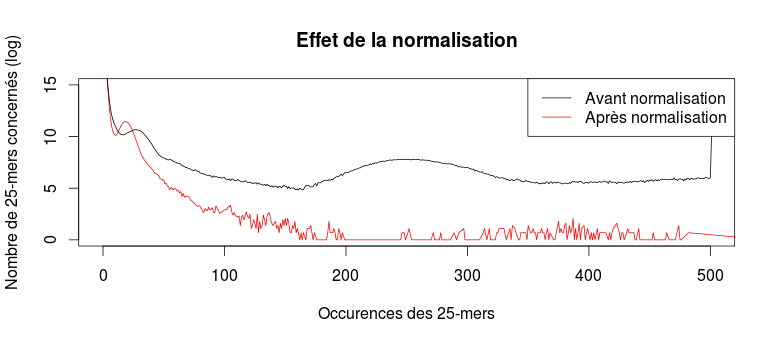
\includegraphics[scale=0.5] {Reduction/norm.png}
   \label{normfilt:1}
 } 
 
 \subfloat[La filtration permet de diminuer le nombre de 25-mers de très faible abondance sans dégrader les données. En effet, le pic d'abscisse 20 constaté à la figure précédente conserve la même forme. Les 25-mers mitochondriaux et chloroplastiques sont donc épargnés par la filtration. Ils apparaissent toujours entre 10 et 30 fois dans le jeu de données.]{
   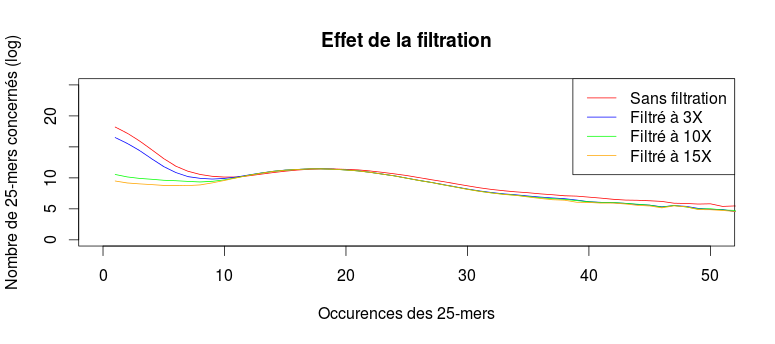
\includegraphics[scale=0.5] {Reduction/filt.png}
   \label{normfilt:2}
 }

\label{normfilt}
\caption{Histogrammes des abondances des 25-mers pour Cvi-0. On représente le nombre y de 25-mers qui apparaissent x fois dans le jeu de données.}
\end{figure}

\subsection{Assemblage}

\subsubsection{Contigage avec Velvet}
\hspace{1.5cm}  \textbf{\small Exemple pour Cvi-0 normalisé à 20X et filtré à 10X}\\

On assemble pour des tailles de k-mer comprises entre 61 et 91, par pas de 10. 

\begin{figure}[!ht]
\centerfloat
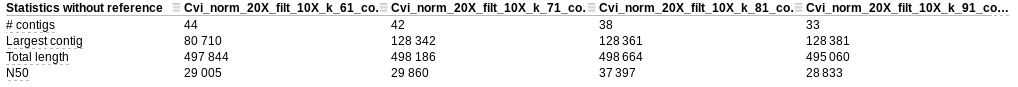
\includegraphics[scale=0.4] {Assemblage/quast.png}
\caption{Les statistiques d'assemblages pour 4 valeurs de k (calculés pour les contigs de taille supérieure à 500 bases)}
\label{quast}
\end{figure}

L'assemblage qui a le plus petit nombre de contigs et la plus grande N50 est l'assemblage réalisé avec k=81. La taille de k-mer optimale va donc se situer autour de 81. On assemble à nouveau le jeu de donnée pour des tailles de k-mer comprises entre 75 et 85, par pas de 2.

On trouve une taille de k-mer optimale de 79. L'assemblage a alors 38 contigs d'au moins 500 bases et une N50 de 39kb. Le contig le plus long a une taille de 149kb. 

Avec Nucmer, on compare les contigs obtenus pour une taille de k-mer de 79 avec le chloroplaste de référence et la mitochondrie de référence. Le plus grand contig de l'assemblage est un contig chimérique. Il s'agit d'un contig chloroplastique qui contient trois grands morceaux d'ADN mitochondrial (de taille 13, 17 et 18kb). Chez la référence, il existe des insertions d'ADN mitochondrial dans le chloroplaste  mais ces insertions sont de petite taille (inférieure à 1kb). Plusieurs grandes insertions d'ADN mitochondrial dans le chloroplaste ont plus de chance de correspondre à un mauvais assemblage qu'à une différence entre les chloroplaste des accessions. 

Pour s'en assurer, on regarde l'assemblage pour k=83, le deuxième meilleur assemblage d'après ses statistiques. Son contig le plus long fait 128kb. Il n'est pas chimérique.

\begin{figure}[!ht]
	\todo[inline]{chloro83: préciser l'assembleur utilisé, les principaux paramètres}
\centerfloat
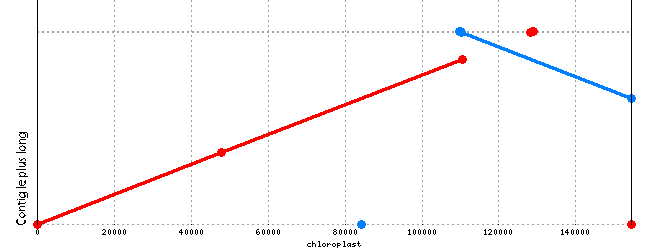
\includegraphics[scale=0.7] {Assemblage/chloro_83.png}
\caption{Graphe de ressemblance entre le plus grand contig obtenu pour k=83 (en ordonnée) et le chloroplaste de référence (en abscisse)\\
Nous n'avons pas représenté les autres contigs afin de ne pas surcharger la figure.}
\label{chloro_83}
\end{figure}

Sur la figure \ref{chloro_83}, on voit que le plus grand contig de l'assemblage s'aligne au chloroplaste de référence dans le sens direct de 0 à 110kb puis dans le sens inverse de 110 à 128kb. Il contient donc la longue région unique du chloroplaste, la première copie de sa région inversée-répétée et la petite région unique du chloroplaste dans le sens inverse (en rouge, bleu et vert sur la figure \ref{schemachloro}). Les trois régions du chloroplaste, qui auraient dû rester distinctes, ont été fusionnées en un seul contig par Velvet. Cet assemblage n'est donc pas bon.\todo[inline]{tu peux déjà mentionner que velvet procede a une étape de scaffolding avec pebble et que tu vas développer l'explication dans la discussion.}

Nous avons testé différents niveaux de normalisation et de filtration mais nous n'avons jamais réussi à obtenir les 3 contigs chloroplastiques attendus. 

\subsubsection{Contigage avec MetaVelvet}
\hspace{1.5cm}\textbf{\small Exemple pour Cvi-0}\\

Nous avons assemblés plusieurs jeux de données ré-échantillonés (qui ne contiennent que la moitié, le tiers, le quart des données etc.) mais les meilleurs résultats ont été obtenus pour les données brutes simplement filtrées à 10X afin de retirer la contamination nucléaire. Nous les présentons ici. 

On effectue la recherche de la taille de k-mer optimale comme précédemment. On choisit k=71. La N50 est alors de 44kb. Il y a 90 contigs d'au moins 500 bases et le contig le plus long fait 85kb. 

\begin{figure}[!ht]
	\todo[inline]{mv: idem dans la légende, préciser l'assembleur utilisé et les principaux paramètres}
\centerfloat

\subfloat[Graphe de ressemblance entre le chloroplaste de référence (en abscisse) et les contigs obtenus (en ordonnée)]{
   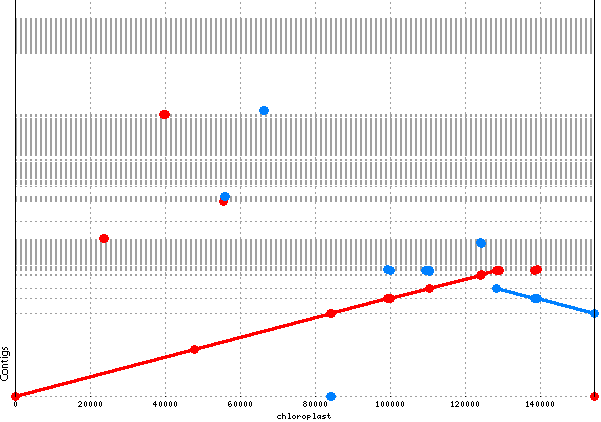
\includegraphics[scale=0.4] {Assemblage/chloro.png}
   \label{mv:1}
 } \hspace{5mm}
\subfloat[Graphe de ressemblance entre la mitochondrie de référence (en abscisse) et les contigs obtenus (en ordonnée)]{
   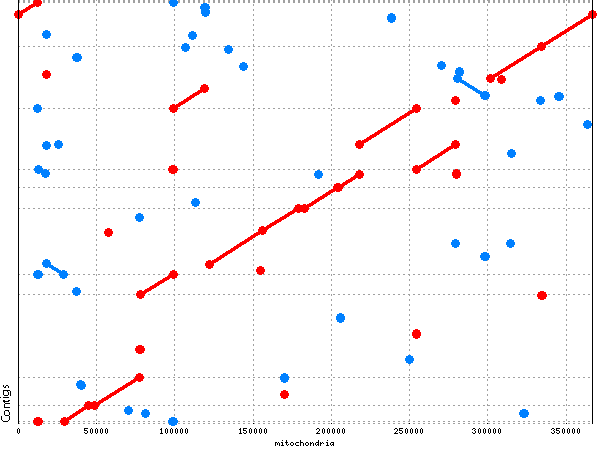
\includegraphics[scale=0.4] {Assemblage/mito.png}
   \label{mv:2}
 }

\label{mv}
\caption{Comparaison entre les contigs obtenus et la référence. Tous les contigs ne figurent pas.}
\end{figure}

En figure \ref{mv:1}, on voit qu'on retrouve dans notre assemblage la longue région unique, la région répétée et la petite région unique du chloroplaste. Ces trois régions correspondent à différents contigs et sont \hlremove{donc}\todo[inline]{il vaut mieux constater le résultat, meilleur que dans le cas de velvet, et ne pas conclure sur autre chose que l'efficacité de l'assembleur. Tu le mentionneras sans doute dans la discussion} bien distinctes. On n'a cependant pas 3 contigs différents mais 5 (la petite région unique et la région répétée sont chacune séparée en deux contigs). 
La figure \ref{mv:2} nous montre qu'on a également dans notre assemblage des contigs qui recouvrent entièrement la mitochondrie de référence. 

\begin{figure}[!ht]
\centerfloat

\subfloat[Les contigs chloroplastiques]{
\begin{tabular}{|l|c|c|c|}
\hline
  & Nom & Taille (bp) & Couverture (X) \\
\hline
Longue région unique & Noeud 1379 &  84093 & 554 \\
\hline
Région répétée & Noeud 8 & 813 & 933 \\
\cline{2-4}
 & Noeud 297 & 15209 & 1117\\
\cline{2-4}
 & Noeud 331 & 10265 & 906 \\
\hline
Petite région unique & Noeud 34 & 3990 & 502 \\
\cline{2-4}
 & Noeud 360 & 13798 & 594 \\
\hline
\end{tabular}

\label{contig:1}
 } \hspace{5mm}
\subfloat[Les contigs mitochondriaux]{
\begin{tabular}{|c|c|c|}
\hline
Nom & Taille (bp) & Couverture (X) \\
\hline
Noeud 7 & 62590 & 60 \\
\hline
Noeud 105 & 21238 & 62 \\
\hline
Noeud 138 & 20691 & 66 \\
\hline
Noeud 222 & 67121 & 56 \\
\hline
Noeud 223 & 455 & 76 \\
\hline
Noeud 227 & 15628 & 53 \\
\hline
Noeud 296 & 44684 & 67 \\
\hline
Noeud 514 & 18462 & 65 \\
\hline
Noeud 541 & 62127 & 60 \\
\hline
Noeud 3153 & 28796 & 61 \\
\hline
Noeud 6544 & 335 & 66 \\
\hline
\end{tabular}

\label{contig:2}
 }

\label{contig}
\caption{Les contigs s'alignant sur le chloroplaste ou la mitochondrie de référence et possédant une couverture cohérente}
\end{figure}

On réaligne les données brutes sur les contigs. On voit que de nombreux contigs présent sur les graphes de ressemblances \ref{mv:1} et \ref{mv:2} possèdent bien la couverture attendue : environ 60X pour la mitochondrie et 560X pour le chloroplaste (le double pour sa région répétée). La liste de ces contigs est donnée dans les tables \ref{contig:1} et \ref{contig:2}. 

Cependant, on trouve également de nombreux contigs qui ne passent pas l'étape de \hlrewrite{consistence}{consistance} interne. Il s'agit : 
\begin{enumerate}
	\item de contigs qui s'alignent sur le noyau de l'accession de référence d'après nucmer ou Blast mais sont extrêmement couverts par les reads \hlrewrite{bruts}{brutes} 

D'après des recherches dans Blast, ces contigs correspondent à des unités répétées d'ADN ribosomique, d'où leur forte couverture.

\item de contigs qui s'alignent sur la mitochondrie ou le chloroplaste de référence d'après nucmer ou Blast mais dont la couverture n'est pas celle qui est attendue

Trois contigs apparaissent plusieurs fois dans le génome mitochondrial de C24 d'après Blast. Ces contigs peuvent également correspondre à des répétitions chez Cvi-0. 

A l'opposé, on a également trois petits contigs qui s'alignent sur la mitochondrie de référence mais dont la couverture est pratiquement nulle. Ces petits contigs, présents chez la mitochondrie de C24, ont peut-être été supprimés du génome mitochondrial de Cvi-0.

\begin{figure}[!ht]
\todo[inline]{inc:2 C'est bizarre, ou bien j'ai mal compris, mais l'hypothèse la plus simple serait peut-etre de considérer que ces contigs sont associés au noyau, Chrm2, vu les niveaux de couverture, contamination qui n'auraient pas pu être éliminés ni par la normalisation/filtration ni par l'assemblage. }
\centerfloat

\subfloat[Des contigs possiblement répetées]{
\begin{tabular}{|c|c|c|}
\hline
Nom & Taille (bp) & Couverture (X) \\
\hline
Noeud 1122 & 2089 & 94 \\ 
\hline
Noeud 1668 & 2163 & 108 \\
\hline
Noeud 2098 & 508 & 90 \\
\hline
\end{tabular}
\label{inc:1}
 } \hspace{5mm}
\subfloat[Des séquences appartenant à la mitochondrie de C24 mais peut-être pas à celle de Cvi-0]{
\begin{tabular}{|c|c|c|}
\hline
Nom & Taille (bp) & Couverture (X) \\
\hline
Noeud 1243 & 251 & 0.6 \\ 
\hline
Noeud 4426 & 230 & 0 \\
\hline
Noeud 4766 & 200 & 0.75 \\
\hline
\end{tabular}

\label{inc:2}
 }

\label{inc}
\caption{Des possibles répétitions et délétions dans le génome mitochondrial de Cvi-0}
\end{figure}

Il existe également des séquences chloroplastiques dont la couverture est trop faible mais on ignore encore pourquoi. 

\end{enumerate}

Nous avons essayé d'utiliser ContigLink pour répérer les contigs mal formés mais sans succès. En effet, si on considère un contig qu'on sait être bien formé, par exemple le noeud 1379 correspondant à la longue région unique du chloroplaste (voir table \ref{contig:1}), on voit que 3629 paires s'alignent sur ce contig avec une bonne taille d'insert et 72692 avec une mauvaise taille d'insert, ce qui représente un \hlrewrite{ration}{ratio} "mauvaises paires"/"bonnes paires" de 0.05. 

\hlcomment{Or, si on étudie maintenant un contig qu'on sait être mal formé, par exemple l'unique contig chloroplastique trouvé par Velvet à la section précédente, on voit que ce mauvais contig est supporté par 7413 "mauvaises paires" pour 132255 "bonnes paires" d'où un ratio de 0.06. On ne peut donc pas utiliser le nombre de paires s'alignant sur un contig avec une taille d'insert incohérente pour distinguer les bons et les mauvais contigs.}{Je dirais que le ratio n'est pas assez informatif en soi et pour être discriminant, il faudrait regarder la localisation/dispersion des paires afin de statuer sur la qualité de l'assemblage des contigs.} 

En revanche, si on visualise l'alignement des données brutes sur ce contig mal formé à l'aide d'IGV, on voit bien qu'on a, à 110 et 128kb, des colonnes de reads dont le compagnon mappe sur le même contig avec une taille d'insert incohérente. Ce qui compte n'est donc pas pas la proportion des "mauvaises" paires par rapport aux "bonnes" mais la localisation des reads de ces "mauvaises" paires. S'ils sont concentrés en un point précis, le contig doit être cassé à cette endroit ; il est donc mal formé. Malheureusement, on ne peut pas visualiser sous IGV tous les contigs. 

\subsubsection{Assemblage avec SGA}
\hspace{1cm}  \textbf{\small Exemple pour Cvi-0 normalisé à 20X et filtré à 10X}\\

\label{sga} En sortie de la phase de contigage, on a un assemblage contenant 65 contigs de plus de 500 bases et dont la N50 est de 13kb. Le contig le plus long fait 46kb. 

Si on réalise le dotplot des contigs contre le chloroplaste de référence, on constate que la longue région unique, la région répétée et la petite région unique du chloroplaste sont bien distinctes même si elles ont été fractionnées en plusieurs contigs. 

On vérifie que la mitochondrie de référence est bien couverte entièrement par certains de nos contigs et que les contigs s'alignant sur la mitochondrie et le chloroplaste de référence ont des couvertures cohérentes.

On peut donc passer à l'étape de scaffolding. On obtient un assemblage final contenant 12 scaffolds, dont le plus long fait 85kb. La N50 est de 26kb. 

\begin{figure}[H]
\centerfloat

\subfloat[Dotplot des scaffolds contre le chloroplaste de référence]{
   \includegraphics[scale=0.3] {Assemblage/chloro_sga.png}
   \label{sga:1}
 } \hspace{5mm}
\subfloat[Dotplot des scaffolds contre la mitochondrie de référence]{
   \includegraphics[scale=0.3] {Assemblage/mito_sga.png}
   \label{sga:2}
 }

\label{sha}
\caption{Comparaison entre les scaffolds obtenus et la référence. }
\end{figure}

Sur le graphe de ressemblance \ref{sga:1}, on voit qu'on a deux scaffolds correspondant aux deux régions uniques du chloroplaste. Les contigs correspondant à la région répétée ont été marqués comme étant des répétitions et écartés de l'assemblage par \textit{sga scaffold}. Pour la même raison, on a sur le graphe \ref{sga:2} des scaffolds qui correspondent aux régions uniques de la mitochondrie avec des gaps qui doivent correspondre aux régions répétées. 


\begin{figure}[H]
\centerfloat

\subfloat[Les scaffolds chloroplastiques]{
\begin{tabular}{|l|c|c|c|}
\hline
  & Nom & Taille (bp) & Couverture (X) \\
\hline
Longue région unique & Scaffold 2 &  84409 & 575 \\
\hline
Petite région unique & Scaffold 10 & 18079 & 600 \\
\hline
\end{tabular}

\label{scaf:1}
 } \hspace{5mm}
\subfloat[Les scaffolds mitochondriaux]{
\begin{tabular}{|c|c|c|}
\hline
Nom & Taille (bp) & Couverture (X) \\
\hline
Scaffold 0 & 14296 & 72 \\
\hline
Scaffold 1 & 18583 & 61 \\
\hline
Scaffold 3 & 11840 & 70\\
\hline
Scaffold 4 & 26808 & 64 \\
\hline
Scaffold 5 & 29698 & 62 \\
\hline
Scaffold 6 & 26539 & 63 \\
\hline
Scaffold 7 & 13731 & 69 \\
\hline
Scaffold 8 & 17754 & 64 \\
\hline
Scaffold 9 & 11367 & 69\\
\hline
Scaffold 11 & 20844 & 70 \\
\hline
\end{tabular}

\label{scaf:2}
 }

\label{scaf}
\caption{Tous les scaffolds s'alignent soit sur le chloroplaste, soit sur la mitochondrie de référence. Ils ont des couvertures proches des valeurs attendues (autour de 60X pour la mitochondrie et de 560X pour le chloroplaste)}
\end{figure}

On réaligne les données brutes sur les scaffolds et on vérifie que les couvertures des scaffolds sont cohérentes (voir tables \ref{scaf:1} et \ref{scaf:2}). Puis, on visualise les alignements pour chaque scaffold avec IGV. On ne repère pas d'endroit précis où des reads dont les compagnons mappent avec des mauvaises tailles d'insert s'accumulent. Il semblerait que les scaffolds soient bien formés. 

%Avec ContigLink, on peut voir qu'aucune "bonne" paire de reads ne supporte de liens entre les scaffolds. 

\subsubsection{Scaffolding avec Bambus2}

On scaffolde les contigs obtenus avec MetaVelvet et décrits en détail à la section \ref{MV_brut}.

On obtient un assemblage final qui comporte 28 scaffolds, dont le plus long fait 85kb. La N50 est de 62kb. 

 
\section{Discussion}

\subsection{Comparaison entre les assembleurs}

Nous avons essayé de comprendre pourquoi Velvet ne nous donne jamais les trois régions distinctes du chloroplaste pour les données normalisées. 

Nous avons remarqué que, même lorsqu'on demande à Velvet ou MetaVelvet de ne pas scaffolder (avec l'option \textit{-scaffolding no}), Velvet/MetaVelvet lance tout de même Pebble, son module de scaffolding. Pebble connecte les contigs uniques en utilisant les informations apportées par les reads pairés. 

Comme dans la section \ref{Velvet_norm}, on utilise Velvet pour assembler les données de Cvi-0 normalisées à 20X et filtrées à 10X pour k=83 mais, cette fois,  en désactivant complètement Pebble (on dit à Velvet que nos données pairées ne le sont pas). 

On obtient un assemblage où les trois régions du chloroplaste sont parfaitement distinctes et représentées chacune par un contig. Cependant, les statistiques de l'assemblage se sont considérablement dégradées. La N50 est passé de 37kb à 16kb. Le nombre de contigs d'au moins 500 bases est passé de 35 à 55. 

On en déduit que, même lorsqu'on lui demande de ne pas scaffolder, Velvet exploite les informations sur les paires si elles sont présentes en utilisant Pebble pour fusionner certaines contigs. Ce premier round de Pebble donne globalement un meilleur assemblage mais il arrive que Pebble fasse des erreurs comme c'est le cas ici pour le chloroplaste. 

Lorsqu'on assemble les données brutes avec MetaVelvet, le premier round de Pebble est également lancé sur chacun des sous-graphes de MetaVelvet. Pourtant, comme nous l'avons vu à la section \ref{MV_brut}, les trois régions du chloroplaste sont distinctes. Donc, Pebble commet l'erreur de relier les trois régions du chloroplaste uniquement pour les données normalisées mais pas pour les données brutes. 

Comme on l'a dit précédemment, Pebble connecte uniquement des noeuds \textbf{uniques}. Or, pour les données normalisées, il fusionne le contig qui correspond à la région répétée du chloroplaste avec les contigs correspondant aux deux régions uniques. Cela signifie que le contig de la région répétée est considéré par Velvet comme étant unique.

Pour distinguer les noeuds uniques des noeuds répétés, Velvet, comme Bambus2 et SGA, calcule la statistique de Myers pour chaque noeud. Il considère que tous les noeuds dont la statistique de Myers est supérieure à 5 sont uniques. \cite{velvetcode}

Malheureusement, Velvet n'écrit pas les résultats de ses calculs dans un fichier. On a donc essayé de répliquer le comportement de Velvet en utilisant le script \textit{sga-astat} pour calculer nous-même la statistique de Myers pour chaque noeud. 

Bien que cette approche soit discutable (on n'est pas sûr que \textit{sga-astat} et Velvet fasse exactement le même calcul), elle donne quand même des résultats intéressants. En effet, on trouve que la statistique de Myers du contig chloroplastique répétée se trouve entre celles des deux contigs chloroplastiques uniques. Or, les contigs répétés doivent forcément avoir une statistique de Myers inférieure à celle des contigs uniques. Si ce n'est pas le cas, on ne peut pas utiliser la statistique de Myers pour distinguer les contigs répétés des contigs uniques. 




\subsection{Comparaison entre les scaffolders}

\subsection{Comparaison entre les accessions}

\section{Conclusion}




\clearpage
\bibliography{biblio}{}
\bibliographystyle{plain}

\end{document}
